\subsection{Product Perspective}
\subsubsection{Scenarios}
\begin{enumerate}
    \item \textbf{Educator creates a battle for a tournament} \\
    The educator who wants to create a battle in a tournament for which he is the creator, or for which he has the permission to create battles.
    The creation of a battle consists of in:
    \begin{itemize}
        \item Set the deadline for registration of teams
        \item Set the deadline for the submission of solutions
        \item Set the minimum and maximum number of students per team
        \item Upload the code kata to the CKB platform
    \end{itemize}
    Once the battle is created, the students registered at that tournament are notified by CKB about the upcoming battle. The CKB platform will also create a new repository on Github for the battle, and will invite the students to fork it.
    \item \textbf{Student invite other students to join the team} \\
    Roberto is a student who wants to participate in a battle. He has already registered in the tournament in which the battle has been created, and he has been notified about the upcoming battle. He wants to invite other students to join his team for the battle. He can do this by sending an invitation to the other students, who will receive a notification about the invitation. The other students can accept or decline the invitation. If they accept, they will be added to the team and they will be able to compete as a team in a battle.
    Even if the students invited have accepted the invitation the partecipation to the battle is not guaranteed since the educator could have set a maximum number of students per team.
    \item \textbf{Student push the solution of the battle to the forked repository} \\
    The team A have been working on the solution for the battle for a while and it seems to be passing all the tests provided in the code kata. Since the time being is before the submission deadline the team push the solution to the forked repository. This will trigger the CKB platform to evaluate the solution and update the score of the team in the battle. In the case that the submission date is after the submission deadline the push will not trigger another evaluation of the solution by the CKB platform.
    \item \textbf{Educator manually updates the score of a team} \\
    Giacomo is an educator who has created a battle for a tournament in which he has been invited by another collegue. Once the submission deadline is expired he wants to manually assess the score of a team to cover all the aspects that the CKB platform cannot evaluate. To do this he access through the CKB platform the battle page and he can see the list of teams that have submitted a solution. He can then manually update the score of a team by clicking on the `Update score' button. This will open a form where he can modify the current score of the team previously evaluated by the platform. Once he is satisfied with the score he can click on the `Save' button to save the new score for the team. The new score will be visible to the team and to the other students subscribed to the tournament.
    \item \textbf{CKB notifies students about the result of the tournament} \\
    When an Educator closes a tournament, the CKB platform will notify all the students subscribed to the tournament about the result of the tournament. The notification will contain the list of the teams that have participated in the tournament and their final score.

\end{enumerate}
\subsubsection{Domain class Diagram}
In \figurename~\ref{fig:domain_class_diagram} is shown the domain class diagram of the CKB platform. This diagram shows the main entities of the system and their relationships.
\begin{itemize}
    \item \textbf{User}: is the main entity of the system. It represents a user of the CKB platform. It can be either a student or an educator.
    \item \textbf{Student}: is a user of the CKB platform. It can participate in tournaments and battles. It can also create teams and invite other students to join them.
    \item \textbf{Educator}: is a user of the CKB platform. It can create and manage tournaments and battles. He can also invite other educators to join a tournament. He also uploads the code kata to the CKB platform for a battle.
    \item \textbf{Tournament}: is a competition between teams of students. It is created by an educator and it can be joined by students. It can contain multiple battles.
    \item \textbf{Battle}: is a competition between teams of students. It is created by an educator and it can be joined by students. It is part of a tournament and it can contain multiple teams.
    \item \textbf{Team}: is a group of students that compete together in a battle. It is created by a student and it can be joined by other students.
    \item \textbf{Invitation}: is a request sent by a student to another student to join a team. It can be accepted or declined by the receiver.
    \item \textbf{Code Kata}: is the description of the problem that the student have to solve in a battle. It contains the description of the software project to be implemented, the test cases that the solution must pass and the build automation scripts.
    \item \textbf{Score}: is the score of a team in a battle. It is calculated by the CKB platform based on the evaluation of the submission of the team. It also adds up the manual score given by the educator. The score assigned to the team, for each battle, is also the score of the students in the tournament.
    \item \textbf{Ranking}: is the ranking of the students in a tournament. It is calculated by the CKB platform based on the score of the students in the battles of the tournament in which they have participated.
    \item \textbf{Repository}: is the repository on Github that contains the code kata and the build automation scripts for a battle. It is created by the CKB platform when a battle is created. It is forked by the teams that want to compete in the battle.
    \item \textbf{Forked Repository}: is the repository forked by a team of students to compete in a battle. It contains the code kata and the build automation scripts for the battle. Each push to the forked repository will trigger the CKB platform to evaluate the submission of the team and update the score of the team.
    \item \textbf{Submission}: is the code that a team of students have implemented for a battle or a subsequent version of a previous submission. It is pushed to the forked repository of the battle by a team member. The CKB platform will evaluate the submission and update the score of the team.
    \item \textbf{Evalutation}: is the evaluation of a submission. It is done by the CKB platform based on the code kata provided by the educator. It is done automatically by the CKB platform when a submission is pushed to the forked repository of the battle. It is also done manually by the educator when he updates the score of a team.
\end{itemize}

\begin{figure}[H]
    \centering
    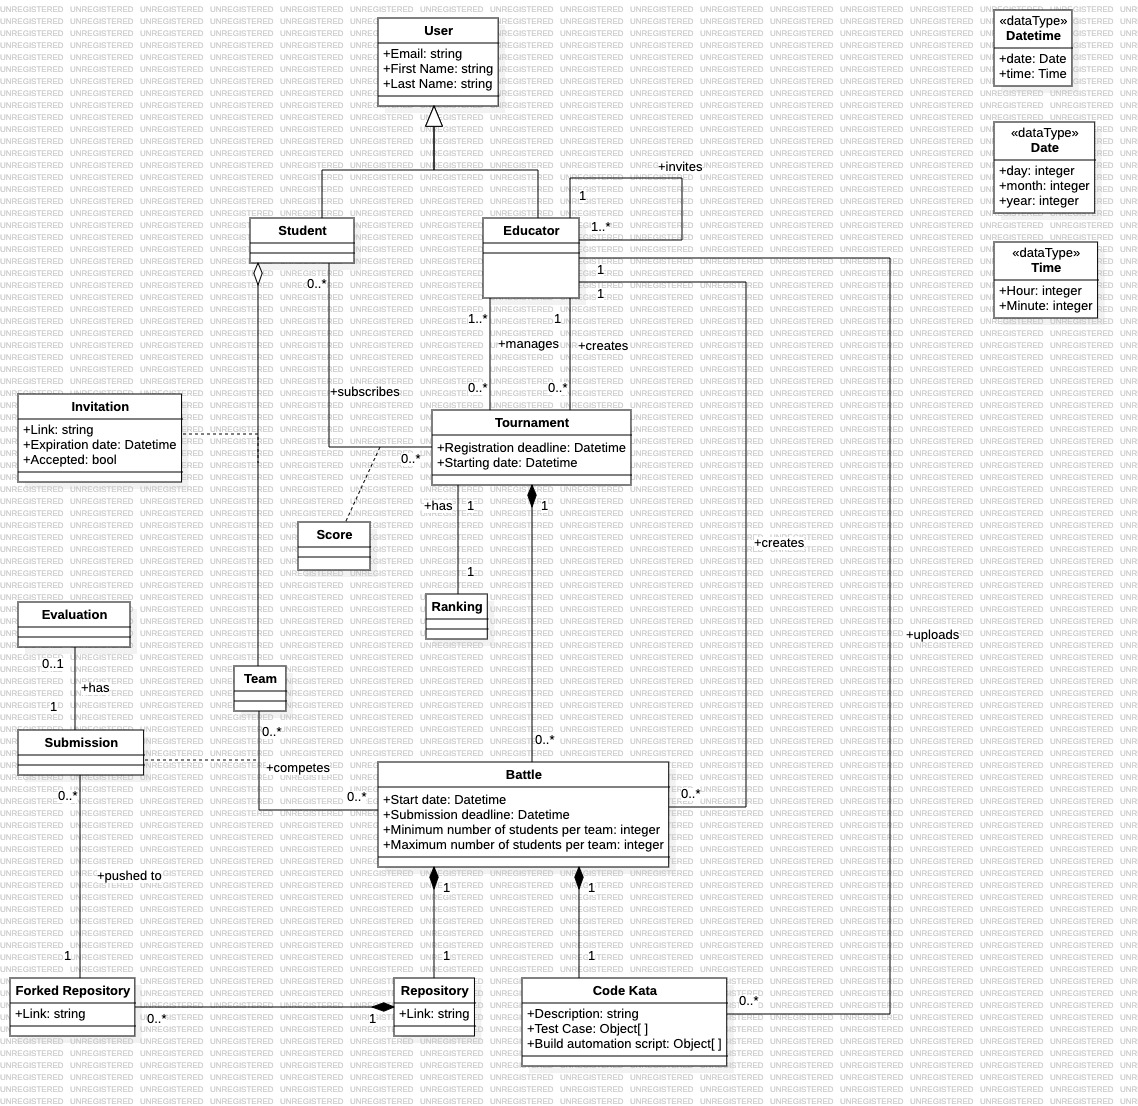
\includegraphics[width=1\textwidth]{Diagrams/DomainClassDiagram.jpg}
    \caption{Domain class diagram}
    \label{fig:domain_class_diagram}
\end{figure}

\subsubsection{Statecharts}

\textbf{Statechart of a Tournament} \\
The statechart in \figurename~\ref{fig:statechart_tournament} shows the possible states of a tournament. A tounament can be in two principal states: ``In Progress'' or ``Closed''. A tournament is in the ``In Progress'' state when it is created by an educator. When the educator closes the tournament, it will be in the ``Closed'' state.
\begin{figure}[H]
    \centering
    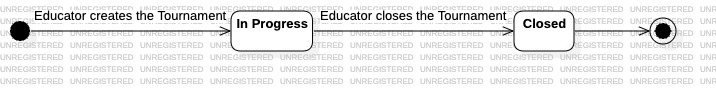
\includegraphics[width=1\textwidth]{Diagrams/TournamentStateChart.jpg}
    \caption{Statechart of a Tournament}
    \label{fig:statechart_tournament}
\end{figure}
\textbf{Statechart of a Battle} \\
The statechart in \figurename~\ref{fig:statechart_battle} shows the possible states of a battle. When the educator creates a battle it will be in initial ``Created'' state. When the date of the \textit{Start date} is passed the battle will be in the ``In Progress'' state. In this state the students can subscribe to the battle and the teams can submit their own solutions. When the \textit{Submission deadline} is passed the battle will be in the ``Consolidation'' state. In this state the educator can manually update the score of the teams. When the educator closes the tournament, it will be in the ``Closed'' state.
\begin{figure}[H]
    \centering
    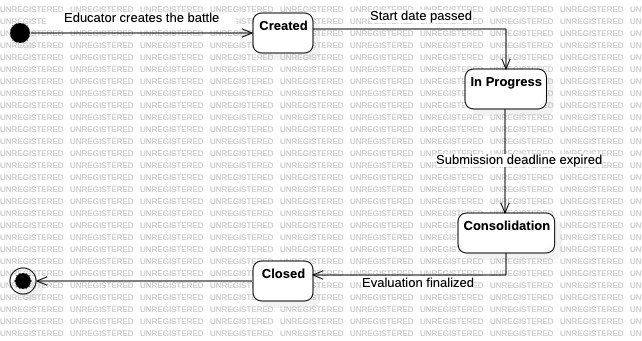
\includegraphics[width=1\textwidth]{Diagrams/BattleStateChart.jpg}
    \caption{Statechart of a Battle}
    \label{fig:statechart_battle}
\end{figure}

\subsection{Product Functions}
\subsubsection{User registration and login}
The CKB platform allows the users to register and login to the platform. The registration is required to access the platform and to use its functionalities. The registration process requires the user to provide a valid email address and a password. The email address will be used to identify the user in the platform \ie{User or Educator}. The password will be used to authenticate the user when he wants to login to the platform. The CKB platform will send a confirmation email to the user to verify the email address. The user will be able to login to the platform only after the email address has been verified.
\subsubsection{Creation of a tournament}
The CKB platform allows the educators to create tournaments. The Educator will be prompted to provide the name of the tournament and the deadline for the registration. When the tournament is created, the CKB platform will send a notification to all the students registered to the platform. The Educator, that has done the creation, will be able to invite other educators to join the tournament.
\subsubsection{Creation of a battle}
The CKB platform allows the educators to create battles. The Educator will be prompted to provide the name of the battle, the deadline for the registration, the deadline for the submission of the solutions, the minimum and maximum number of students per team and the code kata. When the battle is created, the CKB platform will send a notification to all the students subscribed to the tournament. The CKB platform will also create a new repository on Github for the battle, and will invite the students to fork it.
\subsubsection{Creation and joining of a team}
The students in order to compete in a battle must form or join a team. The CKB platform allows the students to create teams by inviting other students to join their team. The student will be prompted to provide the name of the team, as well as the list of the emails of the students that he wants to invite. The CKB platform will send a notification to the invited students. The invited students will be able to accept or decline the invitation. If they accept, they will be added to the team as long as the minimum and maximum number of students per team (set by the educator) is respected.
\subsubsection{Submission and evaluation of a solution}
The students of a team that are competing for a battle can submit their solution to the CKB platform in order to be evaluated. The submission consists of pushing the code that the team has implemented for the battle to the forked repository of the battle previously created by the CKB platform and forked by the team.
The CKB platform will evaluate the submission using the code kata provided by the educator and will update the score of the team.
\subsubsection{Manual update of the score}
The CKB platform allows the educators to manually update the score of a team. After accessing the battle page on the CKB platform, educators can manually adjust a team's score as long as the battle is in the \textit{Consolidation stage}. This feature proves beneficial when evaluating aspects beyond the scope of automatic assessment already done by the platform. On the battle page, educators can view the list of teams that have submitted solutions. By clicking the Update Score' button, a form is opened, allowing the educator to modify the team's current score as assessed by the platform. Once satisfied with the adjustments, clicking the Save' button finalizes the new score.
\subsubsection{Notification of the result of a tournament}
Once an educator closes a tournament, the CKB platform will notify all the students subscribed to the tournament about the result of the tournament. The notification will contain the list of the teams that have participated in the tournament and their final score.
\subsubsection{Creation of the repository to sumbit the solution}
The CKB platform will create a new repository on Github for the battle, and will invite the students to fork it by sending the link of the repository to the students. The repository will contain the code kata provided by the educator and the build automation scripts. The students will be able to push their solution once they have forked the repository and set up the actions to trigger the evaluation of the solution by the CKB platform.

\subsection{User Characteristics}
The CKB platform is designed to be used by two types of users: \textit{Educators} and \textit{Students}.

\subsubsection{Educator}
The Educator is the user that manages tournaments and battles. He is able to invite other educators to join a tournament in order to grant them the permission to create battles for that tournament.
The educator is the user that creates and closes the tournaments and battles (for which he has the permissions to do so in the case he was invited).
He can set restrictions for the battles such as the deadline for the registration of teams, the deadline for the submission of solutions, the minimum and maximum number of students per team. He provides the code kata for the battle. He can also manually update the score of a team. The educator can be looked at as the administrator for a tournament and battles for that tournament. Nevertheless he cannot compete like a student in a tournament or battle.

\subsubsection{Student}
The Student is the user that participates in tournaments and battles. He can team up with other students to compete in a battle by forming teams. He can submit the solution of a battle with his team. He can also compete in multiple battles and multiple tournaments with multiple teams at the same time. The student can be looked at as the competitor in a tournament since the ranking of the tournament is per student. Nevertheless he cannot manage tournaments and battles like an educator.

\subsection{Assumptions, Dependencies and Constraints}

\subsubsection{Regulatory policies}
The CKB platform will store the informations provided by the user, such as the name, surname and email address and informations on forked repositories. This information will not be used for commercial purposes and they will not be shared with third parties.

\subsubsection{Domain assumptions}
This paragraph contains the assumptions that the CKB platform makes about the domain in which it operates. These assumptions are out of the scope of the CKB platform and they are not verified by the platform.

\begin{enumerate}[label=D\arabic*:]
    \item User must have an internet connection
    \item The Student must have a Github account
    \item The Educator must have a Github account
    \item Educator needs to be verified by the CKB platform
    \item Teams must setup the Github actions to trigger the evaluation of the solution by the CKB platform
    \item Student needs to accept the invitation to join a team
    \item Student must be registered to CKB to receive notifications about tournaments
    \item Student must be registered to the tournament to receive notifications about upcoming battles
    \item Educator can evaluate the performance of a student in a battle only if the battle is in the \textit{Consolidation} state
\end{enumerate}